\documentclass{article}
\usepackage{aligned-overset}
\usepackage{amsmath}
\usepackage{amssymb}
\usepackage{bm}
\usepackage[shortlabels]{enumitem}
\usepackage{hyperref}
\usepackage[utf8]{inputenc}
\usepackage{mathtools}
\usepackage{physics}
\usepackage{tabularx}
\usepackage{titling}
\usepackage{fancyhdr}
\usepackage{xfrac}
\usepackage{pgfplots}

\definecolor{light-gray}{gray}{.9}

\pgfplotsset{compat = newest}
\usetikzlibrary{intersections}
\usepgfplotslibrary{fillbetween}

\author{Karsten Lehmann}
\date{SoSe 2021}
\title{Übung 03 Analysis - Weiterführende Konzepte}

\pagestyle{fancy}
\fancyhf{}
\lhead{\thetitle}
\rhead{\theauthor}
\lfoot{\thedate}
\rfoot{Seite \thepage}

\begin{document}

\section*{Uneigentliche Integrale}

\begin{enumerate}[1.]
\item Überprüfen Sie, ob die folgenden uneigentlichen Integrale existieren und
  berechnen Sie gegebenenfalls deren Wert.
  
  \begin{enumerate}[a)]
  \item $\int_0^{\infty} \sin(x)\,dx$

    Der Integrationsbereich ist in diesem Fall nicht beschränkt.
    Um zu prüfen, ob dieser Ausdruck mathematisch sinnvoll ist,
    betrachten wir den Grenzwert
    $\int_0^{\infty} \in(x) \,dx = \underset{\makebox[0pt]{Das setzt die Existenz der Integrale vorraus}}{
      \underbrace{\lim_{b \to +\infty} \int_0^b \sin(x) \,dx}} =
    \lim_{b \to \infty} - \cos(x) {\Big |}_0^b$.

    Das uneigentliche Integral $\int_0^{\infty} \sin(x)\,dx$ existiert nun, wenn
    der Grenzwert $\lim_{b \to \infty} (1 - \cos(b))$ existiert.

    Seien $(b_k)_{k \in \mathbb{N}} = 2 \cdot k \cdot \pi$ und
    $(c_k)_{k \in \mathbb{N}} = 2 \cdot k \cdot \pi + \frac{\pi}{2}$
    zwei Folgen.
    Dann ist
    \[
      \lim_{k \to \infty} 1 - \cos(2 \cdot k \cdot \pi) = 0 \ne
      \lim_{k \to \infty} 1 - \cos\left( 2 \cdot k \cdot \pi + \frac{\pi}{2} \right) = 1
    \]
    und somit existieren sowohl der Grenzwert und daraus folgend auch das
    uneigentliche Integral nicht.

  \item $\int_0^1 \frac{1}{\sin(x)} \,dx$

    Die Funktion $f$ ist in diesem Fall auf dem Integrationsbereich
    nicht beschränkt, denn $\lim_{x \to 0^+} \frac{1}{\sin(x)} = \infty$.
    Das uneigentliche Integral $\int_0^1 \frac{1}{\sin x}\,dx$ existiert nun,
    wenn der Grenzwert $\lim_{a \to +\infty} \int_a^1 \frac{1}{\sin x}\,dx$
    existiert.
    Weiterhin ist $\frac{1}{\sin x}$ auf dem Intervall $[a, 1]$ für
    $a \in (0, 1)$ stetig.

    \textbf{Abschätzung des Grenzwertes durch Substitution}:
    $u(x) = \sin(x), u'(x) =
    \underset{\makebox[0pt]{$\in (0, 1)$, da $x \in [0, 1)$ ist}}{\underbrace{\cos(x)}} =
    \overset{\makebox[0pt]{Trigonometrischer Pythagoras}}{\overbrace{\sqrt{1 - \sin^2(x)}}}
    = \sqrt{1 - u^2}$

    $u'(x) = \frac{du}{dx} = \sqrt{1 - u^2} \Rightarrow dx = \frac{du}{\sqrt{1 - u^2}}$
    \begin{align*}
      \Rightarrow \int_1^a \frac{dx}{\sin x} &= \int_{\sin a}^{\sin 1}
                                               \frac{du}{u \underset{\in (0, 1)}{\underbrace{\sqrt{1 - u^2}}}}
                                               \geq \int_{\sin a}^{\sin 1} \frac{du}{u}
                                               = \ln u {\Big |}_{\sin a}^{\sin 1}\\
                                             &= \ln(\sin 1) - \ln(\sin a)
                                               \overset{a \to +0}\longrightarrow +\infty \\
    \end{align*}
    $\Rightarrow \int_0^1 \frac{dx}{\sin x}$ existiert nicht.

  \newpage
  \label{sec:1c}  
  \item $\int_0^{\infty} \frac{1}{x^2 + 5x + 4} \,dx$

    $f(x) = \frac{1}{\underset{\makebox[0pt]{$> 0$ für $x \geq 0$}}{\underbrace{x^2 + 5x + 4}}}$.
    Außerdem ist die Funktion stetig, damit existieren auch die Integrale.
    Bei Ausdrücken dieser Form müssen zwei Fälle unterschieden werden.
    
    \begin{minipage}[t]{.4\textwidth}
      \[ \swarrow \]
      \[
        \int_0^{\infty} \frac{dx}{\sin x} = \lim_{b \to +\infty} \ln x {\Big |}_1^b = +\infty
      \]
    \end{minipage}
    \hfill
    \begin{minipage}[t]{.4\textwidth}
      \[ \searrow \]
      \[
        \int_0^{\infty} \frac{dx}{x^2} = \lim_{b \to +\infty} -\frac{1}{x} {\Big |}_1^b = 1
      \]
    \end{minipage} \\

    Der Ausdruck $\frac{1}{x^2 + 5x + 4}$ verhält sich ungefähr wie $\frac{1}{x^2}$.
    Dies ist ein erstes Indiz für die Existenz des Grenzwertes.

    $f(x) = \frac{p(x)}{q(x)}, p(x) = 1, q(x) = x^2 + 5x + 4$
    \begin{flalign*}
      q(x) = 0 \Rightarrow x_{1|2} &= -\frac{5}{2} \pm \sqrt{\left(\frac{5}{2}\right)^2 - 4} & \\
      x_1 &= -4, \quad x_2 = -1
    \end{flalign*}
    \begin{flalign*}
      \Rightarrow f(x) &= \frac{1}{(x + 1)(x + 4)} = \frac{a}{x + 1} + \frac{b}{x + 4} =
                          \frac{a(x + 4) + b(x + 1)}{q(x)} && | \cdot q(x)& \\
      \Rightarrow p(x) &= 1 = a(x + 1) + b(x + 4) & \\
      &\text{Durch Einsetzen der Nullstellen folgt:} & \\
      x_1 &= -4 \colon -3a = 1 \Rightarrow a = -\frac{1}{3} & \\
      x_2 &= -1 \colon 3b = 1 \Rightarrow b = \frac{1}{3} & \\
      \Rightarrow f(x) &= \frac{1}{3} \left( \frac{1}{x + 1} - \frac{1}{x + 4} \right) & \\
                       &= \int_0^b f(x)\,dx = \frac{1}{3} \int_0^b \left( \frac{1}{x + 1} - \frac{1}{x + 4} \right) \,dx & \\
                       &= \frac{1}{3} \left( \ln |\underset{>0}{\underbrace{x + 1}}| -
                         \ln|\underset{> 0}{\underbrace{x + 4}}| \middle) \right|_0^b & \\
                       &= \frac{1}{3} \left( \underset{\to 0}{\underbrace{\ln \underset{\to 1}{\underbrace{\frac{b + 1}{b + 4}}}}} -
                         \ln \frac{1}{4} \right) \overset{b \to +\infty}{\longrightarrow} - \frac{1}{3} \ln \frac{1}{4}
                         = \frac{1}{3} \ln 4
    \end{flalign*}
  \newpage                   
  \item $\int_0^{\infty} \frac{x}{(x + 1)^3}$

    $f(x) = \frac{x}{x + 1}^3 = \frac{a}{x + 1} + \frac{b}{(x + 1)^2} + \frac{c}{(x + 1)^3}$.
    Nach der Vorgehensweise von \hyperref[sec:1c]{Aufgabe 1 c)} erhält man
    $p(x) = x = a(x + 1)^2 + b(x + 1) + c$.
    Nach Einsetzen von $x = -1$ folgt $a = 0$, $b = 1$ und $c = -1$.

    \begin{flalign*}
      \int_0^b f(x)\,dx &= \int_0^b \frac{1}{(x + 1)^2} - \frac{1}{(x + 1)^3} = \left( -\frac{1}{x + 1} + \frac{1}{2(x + 1)^2} \middle) \right|_0^b & \\
                        &= \left( -\frac{1}{b + 1} + \frac{1}{2}\frac{1}{(b + 1)^2} \right) - \left( -\frac{1}{2} - \frac{1}{2 \cdot 1} \right)
                          \overset{b \to +\infty}{\longrightarrow} \frac{1}{2}
    \end{flalign*}
  
  \end{enumerate}
  
\item Die Funktion $f \colon [0, \infty) \to \mathbb{R}$ sei auf jedem Intervall
  \label{sec:2}
  $[0, r], r > 0$ Riemann-integrierbar und besitze die folgende Eigenschaft:

  \[
    \forall \epsilon > 0 \,\exists\, R > 0 \,\forall\, s \geq r > R \colon \abs{\int_r^s f(x) \, dx} < \epsilon
  \]

  Beweisen Sie, dass dann das uneigentliche Integral $\int_0^{\infty} f(x)\,dx$ existiert.

  \textit{Lsg.} Nach der Voraussetzung existiert eine Funktion
  $g(z) \coloneqq \int_0^z f(x)\,dx$, $z \geq 0$.
  Wir betrachten nun die Folge $\left(a_n\right)$ mit $a_n \coloneqq g(n)$.

  Sei $\epsilon > 0$ gegeben.
  Dann existiert nach Voraussetzung ein
  \[
    R > 0 \colon \abs{a_n - a_m} = \abs{\int_m^n f(x)\,dx} < \epsilon \forall m, n > R
  \]

  \begin{flalign*}
    \Rightarrow& (a_n) \text{ ist eine Cauchy-Folge} & \\
    \Rightarrow& \exists \lim_{n \to \infty} a_n \eqqcolon I \overset{?}{\Rightarrow} \lim_{z \to \infty} g(z) = I
  \end{flalign*}

  Sei $\epsilon > 0$ gegeben.
  Dann existiert ein $n_0 > R$ mit $\abs{a_n - I} < \frac{\epsilon}{2}$ und
  $\abs{a_n - z} < \frac{\epsilon}{2}$ $\forall n, z \geq n_0$.
  \begin{flalign*}
    \Rightarrow& \, \underset{\makebox[0pt]{$+ a_{n_0} - a_{n_0}$}}{\abs{g(z) \, \underset{\uparrow}{} - I}}
    \leq \abs{g(z) - a_{n_0}} + \abs{a_{n_0} - I} < 2 \cdot \frac{\epsilon}{2} & \\
    \Rightarrow& \, \lim_{z \to \infty} g(z) = I
  \end{flalign*}

\newpage
\item Beweisen Sie, dass das uneigentliche Integral 
  $\int_0^{\infty} \frac{\sin(x)}{x} \,dx$ mit der Eigenschaft aus
  \hyperref[sec:2]{Aufgabe 2} existiert.

  $f(x) = \begin{cases}
    \frac{\sin x}{x} & x \ne 0 \\
    1 & x = 0 \\
  \end{cases}$

  $u(x) = \frac{1}{x}, v'(x) = \sin x, u'(x) = -\frac{1}{x^2}, v(x) = -\cos x$
  \begin{flalign*}
    \underset{\makebox[0pt]{partielle Integration}}{\underset{\uparrow}{\overset{r, s \geq 0}\Rightarrow}}
      \abs{\int_r^s f(x)\,dx} &= \abs{-\frac{\cos x}{x} {\Big |}_r^s - \int_r^s \frac{\cos x}{x^2}\,dx} & \\
                              &= \abs{-\frac{\cos s}{s} + \frac{\cos r}{r} - \int_r^s \frac{\cos x}{x^2}\,dx} & \\
                              &\leq \frac{\abs{\cos s}}{s} + \frac{\abs{\cos r}}{r} + \int_r^s \frac{\abs{\cos x}}{x^2}\,dx
                                \leq \frac{1}{s} + \frac{1}{r} + \int_r^s \frac{1}{x^2} \,dx & \\
                              &= \frac{1}{r} + \frac{1}{s} - \frac{1}{x} {\Big |}_r^s
                                = \left(\frac{1}{r} + \frac{1}{s}\right) + \left( -\frac{1}{s} + \frac{1}{r} \right)
                                = \frac{2}{r} < \epsilon \iff \frac{2}{\epsilon} < r
  \end{flalign*}
  Für $r, s \geq R = \frac{\epsilon}{2} + 1$ gilt damit
  $\abs{\int_r^s f(x)\,dx} < \frac{2}{r} < \epsilon$.

  $\Rightarrow \exists \int_0^{\infty} f(x) \,dx$
  
\item Untersuchen Sie, für welche $s \in \mathbb{R} \setminus \{ 0 \}$ das
  uneigentliche Integral

  \[
    \int_0^{\infty} \frac{1}{x^s + x^{\frac{1}{s}}} \, dx
  \]

  existiert.
\end{enumerate}

\newpage
\section*{Metrische und normierte Räume}

\begin{minipage}[t]{.4\textwidth}
  \textbf{Normierter Raum} \\
  $X$ ist ein Vektorraum.

  $\lVert \cdot \rVert \colon X \to R$ mit
  \begin{enumerate}[(i)]
  \item $\forall x \in X \colon \lVert x \rVert \geq 0$ \\
    $\lVert x \rVert = 0 \Rightarrow x = 0$
  \item $\forall x \in X, \lambda \in K \colon \lVert \lambda x \rVert = \abs{\lambda} \cdot \lVert x \rVert$
  \item Dreiecksungleichung: $\forall x, y \colon \lVert x + y \rVert \leq \lVert x \rVert + \lVert y \rVert$
  \end{enumerate}
  Der normierte Raum ist das Tupel aus dem Vektorraum und der Norm $(X, \lVert \cdot \rVert)$.

  Länge von Vektoren.
\end{minipage} 
\hfill
\vrule
\hfill
\begin{minipage}[t]{.4\textwidth}
  \textbf{Metrischer Raum} \\
  $M \ne \emptyset, d \colon M \times M \to \mathbb{R}$
  \begin{enumerate}[(i)]
  \item $\forall x, y \in M \colon d(x, y) \geq 0$ \\
    $d(x, y) = 0 \Rightarrow x = y$
  \item $\forall x, y \in M \colon d(x, y) = d(y, x)$
  \item Dreiecksungleichung: $\forall x, y, z \in M \colon d(x, y) \leq d(x, z) + d(y, z)$
  \end{enumerate}
  Der metrische Raum ist das Tupel aus dem Vektorraum und der Metrik $(X, \lVert \cdot \rVert)$.

  Abstände zwischen Punkten.
\end{minipage} \\

Alle normierten Räume sind metrische Räume $\Rightarrow d_{\lVert \cdot \rVert} = \lVert x - y \rVert$.

\textbf{Beispiele:}

\begin{minipage}[t]{.4\textwidth}
  \textbf{Normierte Räume} \\
  \begin{itemize}
  \item $(\mathbb{R}, \abs{\cdot})$, $(\mathbb{C}, \abs{\cdot})$, $(\mathbb{R}^N, \norm{\cdot}_p)$
  \item $\norm{x}_p = \qty(\sum_{k = 1}^N \abs{x_k}^p)^{\frac{1}{p}}$ für \\ $1 \leq p \leq \infty$
  \item $\norm{x}_{\infty} = \max\qty{\abs{x_1}, \ldots, \abs{x_N}}$ Maximumsnorm / Supremumsnorm
  \item Kugel um $x$ mit Radius $r > 0 \colon B(x, r) = \qty{y \in X | \norm{x - y} < r}$
  \end{itemize}
\end{minipage} 
\hfill
\vrule
\hfill
\begin{minipage}[t]{.4\textwidth}
  \textbf{Metrische Räume} \\
  \begin{itemize}
  \item $\mathbb{R}^2$ mit Eisenbahnmetrik.
  \item $M$ mit diskreter Metrik
  \item $B(x,y) = \qty{y \in M | d(x,y) < r}$
  \end{itemize}
\end{minipage} \\

\newpage
\begin{enumerate}[1.]
\setcounter{enumi}{3}
\item Sei $\lVert \cdot\, \rVert_p, 1 \leq p \leq \infty$ die $p$-Norm auf $\mathbb{R}^N$
  \begin{enumerate}[a)]
  \item Skizzieren Sie in $\mathbb{R}^2$ die Einheitskugeln für
    $p = 1, 2, \infty$, d.h., skizzieren Sie die Mengen
    \[
      B_p[0, 1] = \left\{ x \in \mathbb{R}^N \middle| \lVert x \rVert_p \leq 1 \right\}
      \text{ bzw. }
      B_p(0, 1) = \left\{ x \in \mathbb{R}^N \middle| \lVert x \rVert_p \leq 1 \right\}
    \]

    \begin{itemize}
    \item $B_1[0, 1] = \qty{x = (x_1, x_2) \in \mathbb{R}^2 | \abs{x_1} + \abs{x_2} \leq 1}$

      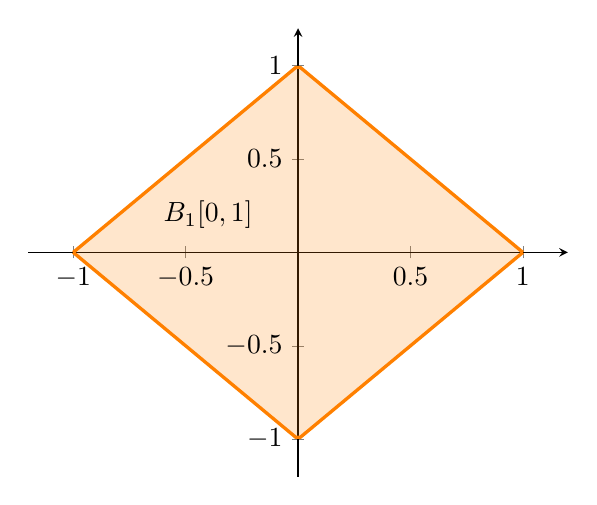
\begin{tikzpicture}
        \begin{axis}[
            axis lines=middle,
            xmax = 1.2,
            xmin = -1.2,
            ymax = 1.2,
            ymin = -1.2,]
          \addplot [
            domain=-1:1,
            samples=100,
            name path=upper,
            very thick, orange]{1 - abs(x)};
          \addplot [
            domain=-1:1,
            samples=100,
            name path=lower,
            very thick, orange]{abs(x) - 1};
          \addplot [
            thick,
            color=orange,
            fill=orange,
            fill opacity=0.2
          ]
          fill between[
            of=upper and lower,
            soft clip={domain=-1:1},
          ];
          \node at (-.4,.2) {$B_1[0,1]$};
        \end{axis}
      \end{tikzpicture}
      
    \item $B_2[0, 1] = \qty{x \in \mathbb{R}^2 | (x_1)^2 + (x_2)^2 \leq 1}$
      
      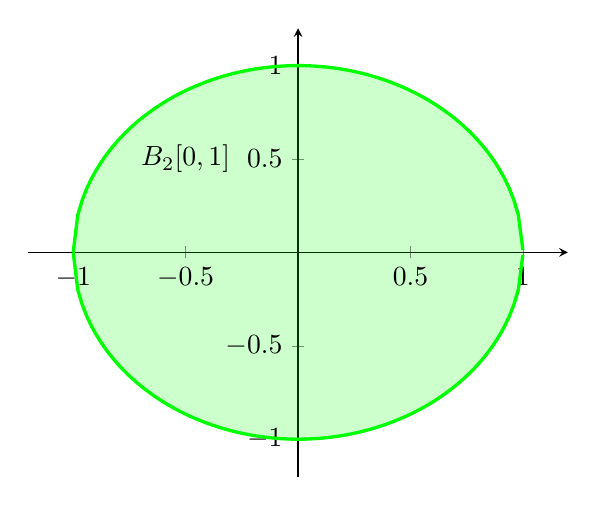
\begin{tikzpicture}
        \begin{axis}[
            axis lines=middle,
            xmax = 1.2,
            xmin = -1.2,
            ymax = 1.2,
            ymin = -1.2,]
          \addplot [
            domain=-1:1,
            samples=100,
            name path=upper,
            very thick, green]{sqrt(1 - x^2)};
          \addplot [
            domain=-1:1,
            samples=100,
            name path=lower,
            very thick, green]{-sqrt(1 - x^2)};
          \addplot [
            thick,
            color=green,
            fill=green, 
            fill opacity=0.2
          ]
          fill between[
            of=upper and lower,
            soft clip={domain=-1:1},
          ];
          \node at (-.5,.5) {$B_2[0,1]$};
        \end{axis}
      \end{tikzpicture}

    \newpage
    \item $B_{\infty}[0, 1] = \qty{x \in \mathbb{R}^2 | \max\qty{\abs{x_1}, \abs{x_2}} \leq 1}$

      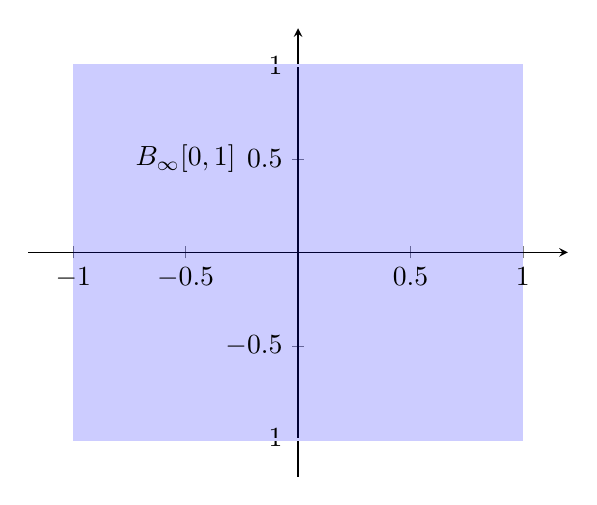
\begin{tikzpicture}
        \begin{axis}[
            axis lines=middle,
            xmax = 1.2,
            xmin = -1.2,
            ymax = 1.2,
            ymin = -1.2,]
          \addplot [
            domain=-1:1,
            samples=100,
            name path=upper,
            very thick, blue!20]{1};
          \addplot [
            domain=-1:1,
            samples=100,
            name path=lower,
            very thick, blue!20]{-1};
          \addplot [
            thick,
            color=blue,
            fill=blue, 
            fill opacity=0.2
          ]
          fill between[
            of=upper and lower,
            soft clip={domain=-1:1},
          ];
          \node at (-.5,.5) {$B_{\infty}[0,1]$};
        \end{axis}
      \end{tikzpicture}
    \end{itemize}

    Bei der Betrachtung der Bilder fällt auf, dass
    \[\begin{aligned}
      B_{\infty}[0,1]   & \geq & B_2[0,1]   & \geq & B_1[0,1] \\
      \norm{x}_{\infty} & \leq & \norm{x}_2 & \leq & \norm{x}_1
    \end{aligned}\]

  \item Beweisen Sie, dass für $1 \leq p \leq q \leq \infty$ und
    $x \in \mathbb{R}^N$ folgende Ungleichungen gelten:
    \[
      \colorbox{orange!50}{$\norm{x}_{\infty}$}
      \leq \colorbox{green!20}{$\norm{x}_q \leq \norm{x}_p$}
      \leq \colorbox{purple!50}{$N^{\sfrac{1}{p}} \norm{x}_{\infty}$}
    \]

    Für $x = 0$ ist alles klar.
    Sei $x \ne 0 \Rightarrow \frac{\abs{x_k}}{\norm{x}_q} \leq 1$ für $k = 1, \ldots, N$.
    Weiter ist $p \mapsto t^p$ für $t \in [0, 1]$ auf $[1, +\infty)$ monoton fallend.
    \begin{align*}
      \overset{q > p}&\Rightarrow \qty(\frac{\abs{x_k}}{\norm{x}_q})^q \leq \qty(\frac{\abs{x_k}}{\norm{x}_q})^p \\
                     &\Rightarrow \sum_{k = 1}^N \frac{\abs{x_k}^q}{\norm{x}_q^q}
                       = \frac{1}{\norm{x}_q^q} \underset{= \norm{x}_q^q}{\underbrace{\sum_{k = 1}^N \abs{x_k}^q}}
                       = 1 \leq \sum_{k = 1}^N \frac{\abs{x_k}^p}{\norm{x}_q^p} = \qty(\frac{\norm{x}_p}{\norm{x}_q})^p
                     && {\Big |} \quad (\ldots)^{\sfrac{1}{p}} \\
                     &\Rightarrow \colorbox{green!20}{$1 \leq \frac{\norm{x}_p}{\norm{x}_q}$}
    \end{align*}
    Für $p = \infty$ existiert ein $k_0$ mit $\abs{x_{k_0}} = \norm{x}_{\infty} = \max\qty{\abs{x_1}, \ldots, \abs{x_N}}$

    \begin{align*}
      \Rightarrow \abs{x_{k_0}}
        &= \colorbox{orange!50}{$\norm{x}_{\infty}$} = \qty\Big(\abs{x_{k_0}}^p)^{\sfrac{1}{p}}
          \leq \qty(\sum_{k = 1}^N \abs{x_k}^p)^{\sfrac{1}{p}} = \norm{x}_p \\
        &\leq \sum_{k = 1}^N \qty\Big(\abs{x_{k_0}}^p)^{\sfrac{1}{p}}
          = N^{\sfrac{1}{p}} \abs{x_{k_0}} =\colorbox{purple!50}{$N^{\sfrac{1}{p}} \norm{x}_{\infty}$}
    \end{align*}
    
  \item Zeigen Sie unter Verwendung der Hölder-Ungleichung, dass für
    $1 < p < q < \infty$ und $x \in \mathbb{R}^N$ die folgende Ungleichung
    gilt:
    \[
      \lVert x \rVert_p \leq N^{\frac{1}{p} - \frac{1}{q} \lVert x \rVert_q}
    \]
  \end{enumerate}


\item Sei $d_2 \colon \mathbb{R}^2 \times \mathbb{R}^2 \to \mathbb{R}$ die
  euklidische Metrik. Für $x, y \in \mathbb{R}^2$ sei
  \[
    d(x, y) \coloneqq \frac{d_2(x, y)}{1 + d_2(x, y)}
  \].
  \begin{enumerate}[a)]
  \item Beweisen Sie, dass $\left( \mathbb{R}^2, d \right)$ ein metrischer
    Raum ist.
  \item Sei $\lVert x \rVert \coloneqq d(x, 0)$.
    Ist dann $\left( \mathbb{R}^2, d \right)$ ein normierter Raum (Begründung)?
  \item Geben Sie die Kugeln $B_d(0, 1)$ und $B_d\left( 0, \frac{1}{2} \right)$
    an. Sind diese Mengen \colorbox{purple!20}{konvex}?
  \end{enumerate}
\end{enumerate}

\end{document}